\documentclass[conference]{IEEEtran}

%+++++++++++++++++++++++++++++++++++++++++++++++++++
\usepackage[pdftex]{graphicx}
\usepackage{amsmath}
\usepackage{eqparbox}
%+++++++++++++++++++++++++++++++++++++++++++++++++++

\begin{document}

%+++++++++++++++++++++++++++++++++++++++++++++++++++
\title{\LARGE Practicum Rough Draft \\ Sentiment Analysis Using Neural and Bag-of-Words Approaches}
\author{\authorblockN{James Barry}
\authorblockA{Dublin City University \\
james.barry26@mail.dcu.ie}}
%+++++++++++++++++++++++++++++++++++++++++++++++++++

\maketitle

\begin{abstract}
This paper implements a binary sentiment classification task on numerous datasets of online reviews. The datasets include the Amazon Fine Food Reviews dataset, the Yelp Challenge Dataset and the IMDb dataset. The paper approaches sentiment classification via two methods: Firstly, a non-neural bag-of-words approach which uses a Support Vector Machine classifier built on top and secondly, using an LSTM RNN. For the LSTM approach, we leverage the use of pre-trained word embeddings such as word2vec and GloVe. We also initialise our own weights from scratch and allow the LSTM to learn the weights itself. The experiment is designed to test the role of word order in sentiment classification by comparing tests where word order is both absent and present. We also include features which give us a greater semantic understanding of the text in the form of pre-trained weights. Our results show that the neural approaches using pre-trained weights perform the best, only by a slight amount. The tests are also carried out on a balanced dataset as well as a randomly distributed dataset.
\end{abstract}

\begin{keywords}
Sentiment analysis, word2vec, GloVe, bag-of-words.
\end{keywords}

\section{Introduction}

Sentiment Analysis is a fundamental task in Natural Language Processing. Its uses are many; from understanding behavioural trends on social media (Bakliwal et al. 2013), gathering insight from user generated product reviews (Jurafsky and Martin, 2000; Pang and Lee, 2008) or even for financial purposes such as for developing trading strategies based on sentiment. The goal of most sentiment classification tasks is to identify the overall sentiment polarity of the documents in question, in our case, online user generated reviews. The academic literature which approaches this task is rich and varied; pioneering approaches include Pang et al. (2002) who use bag-of-words approaches with machine learning algorithms built on top to build a sentiment classifier. The popularity of such bag-of-words approaches is mainly due to their simplicity and efficiency, all the while still achieving very high success. Bag-of-words features are created by viewing the document as a collection of words which in some cases may be linked to an external lexicon containing the sentiment of words. 

Despite their overall high success rates, there exist some downsides to using bag-of-words or n-gram approaches. The main pitfall of such approaches is that that they ignore long-range word ordering such that modifiers and their objects may be separated by many unrelated words (Dai and Le, 2014). As word order is lost, sentences which use the same words will have the exact same representation regardless of the fact that they may have very different semantic meaning. Another key downside to using bag-of-word approaches is that they have very little understanding of the semantics of the words or more specifically, the distances between words in an embedding space (Le and Mikolov, 2014). This is because words are treated as atomic units, resulting in sparse "one-hot" vectors and therefore there is no notion of similarity between words (Mikolov et al. 2013). 

The development of ‘word embeddings’ has advanced many fields within Natural Language Processing. Such methods map words to some high-dimensional embedded word vector space. The corresponding vectors can be used as inputs to enable non-linear learning algorithms such as neural networks (Lochmiller, 2015). The idea of vector representations of words has been further advanced with the development of word2vec (Mikolov et al., 2013) and GloVe (Pennington et al., 2014) which are learned word vector representations based upon unsupervised learning techniques trained on very large corpora. Such representations can encode fundamental relationships between words into a vector space. For example, simple algebraic operations can be performed on the word vectors to yield interesting syntactic relationships between words, such that the vectors "King" - "Man" + "Woman" results in the vector "Queen" (Mikolov et al., 2013). 

Despite the fact that bag-of-words approaches used with machine learning classifiers achieve significant success, the development of word embeddings has allowed us to use more advanced learning algorithms which can remember sequential data such as a Recurrent Neural Network (RNN). Initially, standard RNNs were used for sequence-dependent tasks such as machine translation (Sutskever et al., 2014). RNNs are powerful tools for modeling sequential data but training them by back-propagation through time  can be difficult. Difficulty arises when using RNNs for NLP tasks because the gradients from the objective function vanish after a few time steps (Hochreiter et al., 2001). Indeed, multiple iterations of multiplying the weights of the network can lead to 'vanishing' gradients if the weights are small. Conversely, they will 'explode' if the weight values are large. For such reasons, simple RNNs have rarely been used for natural language processing tasks such as text classification (Dai and Le, 2014). 

In such a scenario we can turn to another model in the RNN family such as the LSTM developed by Hochreiter and Schmidhuber (1997) which are better suited to this task due to the presence  of input gates, forget gates, and output gates which control the flow of information through the network. More recently, neural networks incorporating the LSTM structure have been used for sentiment classification. It is shown that LSTMs achieve very good performance on a variety of document classification tasks with careful tuning of hyperparameters (Dai and Lei, 2014). Such progress in machine learning techniques in recent years has enabled us to use more complex models on large datasets, which typically outperform simple models. A very successful approach is to use distributed representations of words (Hinton et al., 1986). The work of Bengio et al. (2013) and Mikolov (2011) has shown us that using neural network based language models can yield better results than traditional n-gram models.  

\section{Related Literature}

Recurrent neural networks became popular in the 1980s and 1990s with Jordan (1986), Elman (1990) and Rumelhart et al. (1986). They possess the ability to reuse parameters and model sequences over time. The models have a relatively simple architecture, for example, in Elman (1990) there is an input layer for the current feature, a hidden layer which performs some nonlinear computation which also sees its own state from the previous time step and an output layer. Essentially, some form of memory is achieved by the state of the hidden layer. 

While initially an exciting model, it became known that there were some drawbacks with RNNs particularly in their ability to train, especially with stochastic gradient descent and backpropagation because of the vanishing/exploding gradient problem (Hochreiter, 1991; Bengio, 1994). An important development which helped deal with these issues was the LSTM RNN architecture developed by Hochreiter and Schmidhuber (1997) which added further architecture to the simple recurrent neural network which include neurons with input gates, forget gates and output gates which allowed the models to achieve greater memory by controlling the flow of information to hidden neurons. Their success was shown in NLP tasks such as hand writing recognition by Graves and Schmidhuber (2009). Today RNNs are used for many tasks such as speech recognition, machine translation, handwriting recognition and many other sequential problems.

Alongside the development of more sophisticated RNNs, a big development in NLP tasks was the development of word embeddings. Despite their recent fame, they are not necessarily a recent phenomena. Hinton et al. (1986) and Elman (1991) showed that simple neural networks can be used to obtain distributed representations of words. Collobert and Weston (2008) achieved great success in using deep neural networks for the same purposes. Collobert (2011) induced useful word embeddings by applying a convolutional network architecture to a language modeling task trained using a large amount of unlabeled text data. These embeddings improve the generalisation performance on many NLP tasks, in particular, part-of-speech tagging and named entity recognition. The general idea of how their model works is that a word and its context is a positive training example, whereas when a random word is placed in that same context, this gives us a negative training example: For example, a good training example would be "cat chills on a mat" and a bad example - "cat chills Jeju a mat". A neural network model gives a greater score for the real word in the sample than a random word in the same context. Other approaches for creating word embeddings using neural networks include Bengio et al. (2003) and  Turian et al. (2010) who  use deep learning models to represent words as a dense vector. Such word embeddings enable an understanding of the degree of similarity between words and also get rid of the problem where we have sparse one-hot vectors. 

More recently, for learning word embeddings, Mikolov et al., (2013) and Pennington et al. (2014) developed the very popular word embeddings word2vec and GloVe respectively. Mikolov et al. (2013) develop simple architectures such as continuous-bag-of-words (CBOW) and Skip-Hram to find distributed representations of words. Like the quote, "You shall know a word by the company it keeps by Firth (1957), the models gain understanding of words in a corpora by analysing the co-occurrences of words over a large training sample. Word2vec is much faster and more accurate than previous neural network based approaches, and speeds up training from previous methods significantly. Word embeddings have become really popular as the  features can easily be used in classifiers to boost the performance on many NLP tasks.

Studies which use neural network architectures include Socher et al. (2011) who use a semi-supervised approach using recursive autoencoders for predicting sentiment distributions. The model learns vector space representations for multi-word phrases and possesses the ability to understand the recursive nature of sentences. Socher et al. (2013) highlight that understanding compositionality in tasks such as sentiment detection requires richer supervised training resources and more powerful models of composition. To fulfill such criteria, the authors introduce a Sentiment Treebank which includes sentiment labels for over 215,000 phrases. They also introduce a Recursive Neural Tensor Network, which when trained on the new Treebank, outperforms all previous methods on several metrics and forms a state of the art method for determining the positive/negative classifications of single sentences. Li et al. (2015) evaluate the effectiveness of recusive and recurrent neural networks on five NLP tasks including sentiment classification. Kalchbrenner et al. (2014) use convolutional neural networks. The effectiveness of recursive neural network and recurrent neural network on five NLP tasks including sentiment classification. Kalchbrenner et al. (2014) use convolutional neural networks. Dai and Lei (2014) perform a document classification task across a variety of datasets as well as a sentiment analysis task. They found that LSTMs pretrained by recurrent language models or sequence autoencoders are better than LSTMs initialised from scratch. Le and Mikolov (2014) introduce Paragraph Vector to learn document representation from semantics of words.

Concerning sentiment classification, Pang et al. (2002) use three standard algorithms: Naive Bayes classification, maximum entropy classification and a support vector machine to compare their performance in determining sentiment classification on document data (IMDb movie reviews). The authors incorporated a standard bag-of-features framework, which included good indicator words for positive and negative sentiment. Their results showed that machine learning techniques outperformed that of human generated baselines. Despite the success such approaches one problem with bag-of-words methods is that they are unable to deal effectively with negation. For example if they see words like "great" or "inspiring" in a review, it elicits a strong positive sentiment. However, if the actual sentence was "the cast was not great, nor was the movie inspiring" it has a completely different meaning which the models will fail to pick up. To overcome such difficulties as negation, researchers such as Turney (2002), developed hand-written algorithms which can reverse the semantic orientation of a word when it is preceded by a negative word. Turney develops a simple unsupervised learning algorithm for classifying reviews as recommended or not recommended.  The algorithm uses a written review as the input and produces a classification (recommended or not recommended) as the output. Turney first uses a part-of-speech tagger to identify phrases in the text that contain adjectives or verbs and then estimates the semantic orientation of the phrases. While such algorithms are an important development to handle things like negation, it can be very time consuming to develop heuristically designed rules which may not be able to deal with the multiple scenarios prevalent across human language. 


\section{Data}

Our datasets include the Amazon Fine Food Reviews dataset, the Yelp Challenge dataset and the IMDb dataset, all of which contain a series of reviews and labeled ratings. For this project, as it is a sentiment classification task, only the data containing raw text reviews and their equivalent rating were parsed. 

\begin{figure}[ht!] %!t
\centering
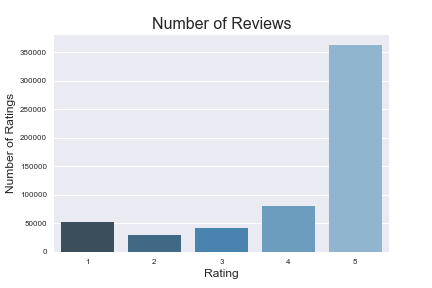
\includegraphics[width=3.45in]{aff.png}
\caption{ Distribution of Ratings Amazon}
\label{picture}
\end{figure}

The Amazon Fine Food Reviews Dataset contains 568,454 reviews. The number of words in the dataset is 45,947,710. The number of sentences is 2,834,359. The average number of sentences is: 4.986083. 

\begin{figure}[ht!] %!t
\centering
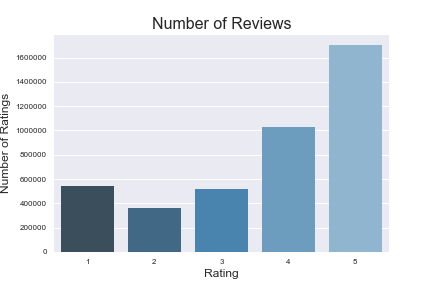
\includegraphics[width=3.45in]{yelp.png}
\caption{ Distribution of Ratings Yelp}
\label{picture}
\end{figure}

The Yelp Challenge Dataset contains numerous files containing data from the Yelp website. We use the Yelp Academic Reviews dataset, which contains written reviews of listed businesses. The dataset contains over 4 million reviews and we parse data from two fields: "stars" and "text", where "stars" is the customer's rating from 1 to 5 and "text" is the customer's written review. The number of reviews in the dataset are 4,153,150. Out of a sample of 100,000 reviews: The number of sentences are: 829,165. The number of words are: 11,569,896. The average number of sentences are: 8.29.

\begin{figure}[ht!] %!t
\centering
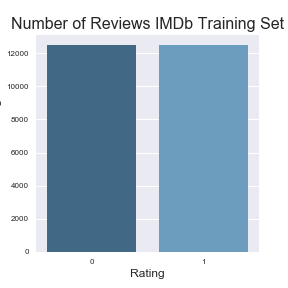
\includegraphics[width=3.45in]{imdb.png}
\caption{ Distribution of Ratings IMDb}
\label{picture}
\end{figure}

Our final dataset is the IMDb dataset. The dataset contains movie reviews which are already split evenly between positive and negative review labels. The dataset contains 50,000 reviews which are split into 25,000 training and 25,000 test sets. There also exists an additional 50,000 unlabeled documents for unsupervised learning. In the labeled training/testing sets, negative reviews are those which have a score below 5 out of 10, whilst a positive review has a score of over 6 out of 10. As a result, neutral reviews are not included in the training/testing sets. In the unsupervised set, reviews of any rating are included and there are an even number of reviews greater than 5 and less than or equal to 5. The dataset consists of three columns: id, sentiment (binary 1 or 0) and review, the raw text review.  

For the pre-trained weights used in the embedding layer of our LSTM model, we used word2vec weights and GloVe (will elab on how they were trained). 

\subsection{Data Processing}

The ratings in the Amazon and Yelp datasets were turned into binary positive and negative reviews where negative labels were assigned to ratings of 2 stars and below. Positive labels were assigned to ratings of 4 stars and above. Neutral, 3-star reviews were excluded so that our data would be highly polarised.

\section{Approach}

A long term goal for NLP and AI research involves developing machines which have the ability to understand language. If a human were asked to carry out a sentiment classification task, it would be presumed that they would carry out the task in a sequential, bottom-up fashion whereby they analyse the semantic relationship of the words and sentences overall rather than declaring the polarity of the review based on individual words. This motivates us to carry out this test: firstly to use traditional bag-of-words methods with an SVM classifier as a baseline, and secondly, to mimic a more human approach, using word order and features which have more intelligent understanding of semantics such as pre-trained word embeddings. 

As mentioned in the Introduction, traditional methods of sentiment analysis such as Bag of Words models, disregard the order of words, therefore these experiments will aim to compare various models which can incorporate sequential data, such as a recurrent neural network versus the bag-of-features model. Here the input sentence can be viewed as a sequence of tokens, rather than an unordered bag of tokens. 

\subsection{Model Design: Support Vector Machine}

A Support vector machine is (maybe see Pang (2002) for definitions and formulas).

\subsection{Approach 1:} 

For the bag-of-words approach, the reviews were cleaned via a text-processing algorithm to remove any unwanted characters such as html links or numbers and retrieve only raw text. The next stage is to convert the words so that they have a numeric representation which can be used in machine learning models. The Bag of Words model learns a vocabulary from all of the words in the documents. It then models each document by counting the number of times each word appears. Considering the datasets contain a large volume of reviews, resulting in a large vocabulary, to limit the size of the feature vectors we choose a maximum vocabulary size of 5000. Once the feature vectors were created, we could then use a support vector machine to classify the text as positive. 


\subsection{Model Design: LSTM}

Maybe use formulas on Chris Olah's LSTM blog.

\subsection{Approach 2: }

For the second approach, we use LSTM recurrent networks because they are generally better than traditional recurrent neural networks for learning trends in sequential data. This is due to their unique architecture of having input gates, forget gates and output gates. The test is carried out as follows, a user’s review (a sequence of words) is used as inputs to our model which then outputs the category of the highest softmax score as the class label, i.e. based on the input, is the review positive or negative? 

As with Approach 1, we use an algorithm to process the text to remove any unwanted characters. We then convert all text samples in the dataset into sequences of word indices which essentially involves converting the word to an integer ID for the word. Essentially, we convert words from each text document into a sequence of vectors which can be used in our model. Each resulting sequence of vectors will be a separate data sample used an an input into the LSTM. The LSTM will then process all vectors in that sequence and it will output a vector with a probability of the text belonging to a positive or negative category. 

For this study, we only consider the top 20,000 most common words and we truncate the sequences to a maximum length of 1000 words. Once the words are converted into integers, we can prepare an “embedding matrix” which will contain at index i, the embedding vector for the word of index i in our word index. These embedding matrices are loaded into a Keras embedding layer. We will build an LSTM RNN ending in a softmax output to classify the review. This process is carried out with 3 variations: we will use word embeddings which are a family of natural language processing techniques aimed at mapping semantic meaning into a geometric space (Chollet). This is achieved by allocating a numeric vector to every word in a dictionary. By doing so, the distance (e.g. cosine distance) between any two vectors will capture part of the semantic relationship between the words. The geometric space formed by these vectors is called an embedding space. Word embeddings are computed by applying dimensionality reduction techniques to datasets of co-occurrence statistics between words in a corpus of text. This can be done via neural networks, the "word2vec" technique, or via matrix factorization. For this study we use pretrained word2vec and GloVe embeddings.  We will be using GloVe embeddings GloVe stands for "Global Vectors for Word Representation". It's a somewhat popular embedding technique based on factorizing a matrix of word co-occurence statistics.

We  also test how well we would have performed by not using pre-trained word embeddings, but instead initialising our Embedding layer from scratch and learning its weights during training.

Talk about the various tests you will do: 

Development set which is used to tune the parameters of the models to prevent over-fitting and improve accuracy. 

Word2vec initialised on own corpora

Different types of dataset - random sample of size n, evenly distributed dataset of similar size and larger dataset. 



\section{Results}

\begin{tabular}{ |p{3cm}||p{3cm}|p{3cm}|p{3cm}|  }
 \hline
 \multicolumn{4}{|c|}{Model Results} \\
 \hline
 Model Type& Amazon & Yelp & IMDb\\
 \hline
 Naive Bayes tf idf &   AS  & ASM&016\\
 BoW SVM   & AF    &AFG&   004\\
 BoW SVM bigram &   AX  & ALA   &248\\
 LSTM Word2Vec &AL & ALB&  008\\
 LSTM GloVe    &DZ & DZA&  012\\
 LSTM own weights &   AS  & ASM&016\\
 Ensemble method & AD  & AND   &020\\
 LSTM Word2vec* &   AS  & ASM&016\\
 \hline
\end{tabular}


The results show - will update with figures (these values don't mean anything yet!)

\section{Conclusion}

In this study we have compared x approaches, firstly using bag-of-words approach. Secondly an LSTM RNN which leverages pre-trained weights such as word2vec and glove as well as learning its own weights. Also mention other methods such as ensemble, word2vec initialised on own corpora, balanced v randomly sampled dataset.

%\section*{Acknowledgment}
%For the Summary paper submission only, no %acknowledgements are allowed. 

\section{References}

Will build .bib file in due course 

Bo Pang, Lillian Lee and Shivakumar Vaithyanathan (2002)

T. Mikolov, A. Deoras, S. Kombrink, L. Burget, J. Cernock ˇ y. Empirical Evaluation and Com- ´
bination of Advanced Language Modeling Techniques, In: Proceedings of Interspeech, 2011.

Y. Bengio, R. Ducharme, P. Vincent. A neural probabilistic language model. Journal of Machine
Learning Research, 3:1137-1155, 2003.

Distributed Representations of Sentences and Documents
Quoc Le
Tomas Mikolov
[Rumelhart et al. 1986]

\end{document}